\documentclass[en,t,navbarkit]{sdqbeamer}

\usepackage{amssymb} %% For \backprime
\usepackage{multicol}
\usepackage{mathpartir}

%\usepackage{mathpartir}
\usepackage{graphicx}

\usepackage{tikz}
\usetikzlibrary{arrows.meta,positioning,calc,fit}

\usepackage[style=authoryear,backend=bibtex]{biblatex}
\bibliography{lean}

\usepackage[T1]{fontenc}
\usepackage[english]{babel}
\usepackage{booktabs}
\usepackage[normalem]{ulem}
\usepackage{fontspec}
\setmonofont[RawFeature=-calt,Scale=MatchLowercase]{Iosevka}
%\newfontfamily\lc[Scale=MatchLowercase]{Iosevka SS09}

\usepackage{minted}
\definecolor{codebg}{rgb}{0.95,0.95,0.95}
\setminted{bgcolor=codebg,breaklines}
\usemintedstyle{tango}
\newmintinline[lean]{theorem.py:LeanLexer -x}{bgcolor=white}
\newminted[leancode]{theorem.py:LeanLexer -x}{fontsize=\footnotesize}

\usepackage{newunicodechar}
\newfontfamily{\freeserif}{DejaVu Sans}
\newunicodechar{ℕ}{\freeserif{ℕ}}
\newunicodechar{ℝ}{\freeserif{ℝ}}
\newunicodechar{ₐ}{\freeserif{ₐ}}
%\newunicodechar{₁}{\freeserif{₁}}
%\newunicodechar{∈}{\freeserif{∈}}
\newunicodechar{𝓞}{\ensuremath{\mathcal{O}}}
\newunicodechar{∉}{\freeserif{∉}}
%\newunicodechar{Π}{\freeserif{Π}}
%\newunicodechar{→}{\freeserif{→}}
\newunicodechar{⦃}{\freeserif{⦃}}
\newunicodechar{⦄}{\freeserif{⦄}}
%\newunicodechar{∧}{\freeserif{∧}}
%\newunicodechar{∨}{\freeserif{∨}}
%\newunicodechar{⊢}{\freeserif{⊢}}
\newunicodechar{⊑}{\freeserif{⊑}}
\newunicodechar{ₚ}{\freeserif{ₚ}}
\newunicodechar{∘}{\freeserif{∘}}
\newunicodechar{ₗ}{\freeserif{ₗ}}
\newunicodechar{∪}{\freeserif{∪}}
\newunicodechar{⋃}{\freeserif{⋃}}
\newunicodechar{𝓸}{\ensuremath{o}}
\newunicodechar{⊆}{\freeserif{⊆}}
\newunicodechar{≼}{\freeserif{≼}}
\newunicodechar{≃}{\freeserif{≃}}
\newunicodechar{✝}{\freeserif{✝}}

% https://github.com/gpoore/minted/issues/220
\AtBeginEnvironment{snugshade*}{\vspace{-0.4\FrameSep}}
%\AfterEndEnvironment{snugshade*}{\vspace{-0.8\FrameSep}}

% https://tex.stackexchange.com/questions/343494/minted-red-box-around-greek-characters
%\makeatletter
%\AtBeginEnvironment{minted}{\dontdofcolorbox}
%\def\dontdofcolorbox{
\renewcommand\fcolorbox[4][]{#4}
%}
%\makeatother

\titleimage{logo}
\grouplogo{}
\groupname{IPD Snelting}

\title{Gotta Prove Fast}
\subtitle{Building an Ecosystem for Effortless Native Compilation of Tactics}

\author{Sebastian Ullrich}
\date{2022/01/06}

\begin{document}

\KITtitleframe

\begin{frame}{The Lean 4 Project~\textcolor{gray}{\small[de Moura \& Ullrich 2021]\nocite{demoura2021lean}}}
  %   Lean 4 is the upcoming version of the Lean theorem prover \& programming language
  \begin{centering}
    \vfill

  Provide a fully extensible theorem proving frontend

  % ... by way of an expressive, hygienic macro system
  \vfill

  Erase the boundary between built-in and custom macros/tactics/...
  \\
  by reimplementing >75\% of Lean in Lean itself

  \vfill

  Make Lean an efficient, general-purpose programming language

  \vfill
  \end{centering}
\end{frame}

%\begin{frame}{Compiling Tactics -- \emph{Why?}}
%  \begin{itemize}
%    \item write your own simplifier, etc.
%    \item even with external solvers, efficient internal ones still important for proof reconstruction, e.g.\ Sledgehammer/metis
%    \item Gabriel Ebner built a superposition solver in Lean 3, but interpreter performance insufficient
%  \end{itemize}
%\end{frame}

\begin{frame}{Compiling Tactics -- \emph{How?}}
  \pause
  \begin{itemize}
    \item A Just-In-Time Compiler? LLVM JIT?
          \begin{description}
            \item[+] run tactic with native performance in the same file
            \item[--] re-compile tactic in every importing file...?
            \item[--] would first need a true LLVM backend
          \end{description}
          \pause
    \item reuse Ahead-Of-Time toolchain for stand-alone Lean programs
          \begin{description}
            \item[+] much simpler... hopefully!
            \item[+] benefits stand-alone use case as well
            \item[--] should probably use the interpreter in the same file
            %\item[--] compiler toolchains are complicated!
          \end{description}
  \end{itemize}
\end{frame}

\pgfdeclarelayer{back}
\pgfsetlayers{back,main}

\begin{frame}{Lean 4 Compilation Pipeline}
  \begin{center}
    \begin{tikzpicture}[>=stealth, thick, nodes={rounded corners, minimum height=2em}, level distance=15mm, sibling distance=30mm]
      \node[draw] (elaborator) {elaborator}
      child[->] {
        node[draw] (kernel) {kernel}
        edge from parent node[left] {core term}
      }
      child[->] {
        node[draw] {compiler} [sibling distance=20mm]
        child[->] {
          node[draw] (interpreter) {interpreter}
          edge from parent node[left] {IR}
        }
        child[->] {
          node[draw] {C emitter}
          child[->] {
            node[draw] (clang) {clang}
            child[->] {
              node {}
              edge from parent node[right] {.exe}
            }
            edge from parent node[right] {.c}
          }
          edge from parent node[right] {IR}
        }
        edge from parent node[right] {core term}
      };
      \draw[->,bend left=10] (interpreter) to node[sloped,above=-1mm] {tactic} node [sloped,below=-1mm] {exec} (elaborator);
      \uncover<2->{
      \draw[->,color=kit-green] (clang) to node[below] {.dll} (interpreter);
      }
      \begin{pgfonlayer}{back}
      \uncover<3>{
        \node[fit=(kernel),fill=blue!50,draw=blue,thick,rounded corners=0pt] {};
      }
      \end{pgfonlayer}
    \end{tikzpicture}
  \end{center}
  \vspace{-1cm}
  \uncover<3>{NB: The \textcolor{blue}{Trusted Code Base} is unaffected!}
\end{frame}

\begin{frame}{So You Want to Build a Native Binary}

  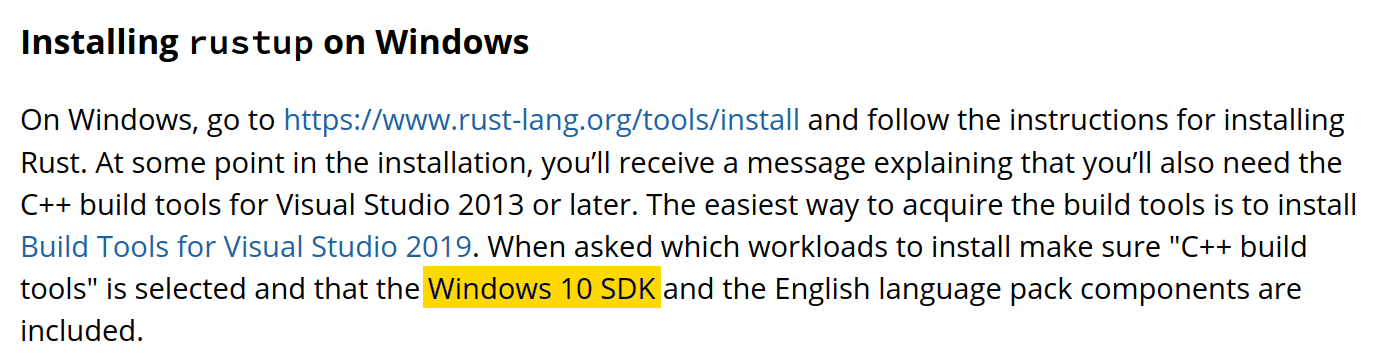
\includegraphics[width=0.8\textwidth]{rust2.png}
  \pause
  %\only<2-3>{
  %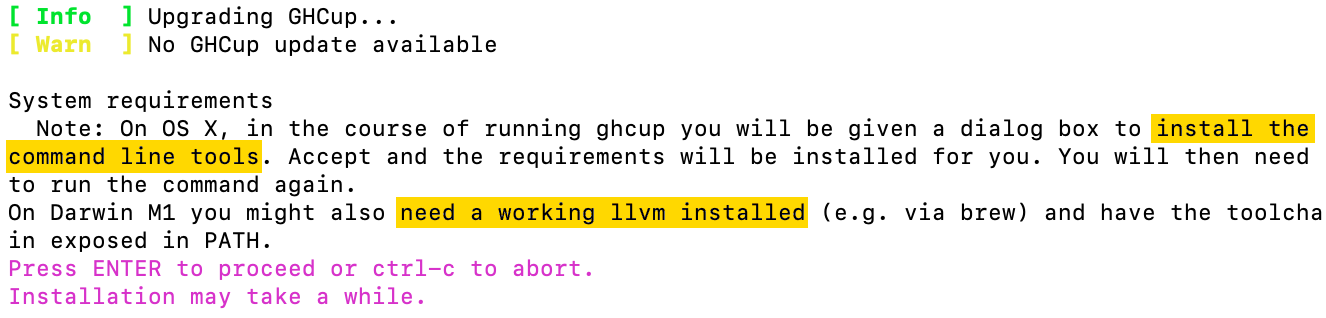
\includegraphics[width=0.8\textwidth]{haskell2.png}

  \only<2>{We need effortless setup \emph{not requiring root}!}
  %}
  \pause
  %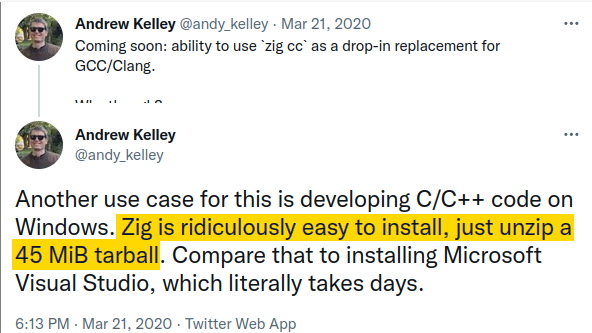
\includegraphics[width=0.6\textwidth]{zig2.png}
  The \emph{Zig} language manages to provide small, self-contained toolchains for many platforms
  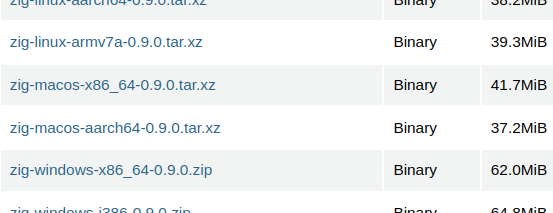
\includegraphics[width=0.4\textwidth]{zig3}
\end{frame}

\begin{frame}[fragile]{Assembling a Native Compilation Pipeline}
  %goal: a common, zero-setup pipeline for all platforms
  %\vfill

  LLVM comes with many necessary parts:
  \begin{itemize}
    \item a C compiler
    \item basic C headers
    \item a runtime library
    %\item a C++ stdlib
    \item a linker (good macOS support since LLVM 13)
    \item a static archiver
  \end{itemize}

  \vspace{3mm}
  \pause

  It does not help at all with assembling
  \begin{itemize}
    \item the above with \emph{reasonable} runtime dependencies
    \item a libc
          \begin{itemize}
            \item Linux: bundle older glibc for compatibility
            \item macOS: bundle \texttt{libSystem.tbd} from SDK/Nixpkgs
            \item Windows:~\pause\verb!cp /clang64/x86_64-w64-mingw32/lib/lib{m,bcrypt,mingw32,moldname,mingwex,msvcrt,pthread,advapi32,shell32,user32,kernel32,ucrtbase}.*!
          \end{itemize}
  \end{itemize}
\end{frame}

\tikzset{lean/.style={draw,fill=white}}
\tikzset{dll/.style={draw,gray,thick,rounded corners=0pt,align=right,inner sep=2pt}}
\tikzset{nameddll/.style={dll,inner sep=7pt,xshift=5pt,yshift=-5pt}}
\tikzset{dllname/.style={above left,gray,yshift=-1.5mm,font=\scriptsize}}
\tikzset{hide on/.code={\only<#1>{\color{fg!0}}}}

\begin{frame}[fragile]{Compiling Tactics -- \emph{Where?}}
  \hspace{3cm}
    \begin{tikzpicture}[>=stealth, thick, nodes={rounded corners, minimum height=2em}, level distance=15mm, sibling distance=30mm]
      \node (deps) {...}
      child[<-] {
        node[lean] (tac) {\lean{elab "my_tac" : tactic => ...}}
        child[<-] {
          node[lean] (use1) {\lean{... by my_tac}}
        }
        child[<-] {
          node[lean] (use2) {\lean{... by my_tac}}
        }
      }
      child[sibling distance=60mm,hide on=-2] {
        node[lean] (tac2) {\only<3->{\lean{elab "my_tac2" ...}}}
        edge from parent[draw=none]
      };
      \only<3->{
        \draw[<-] (deps) to (tac2);
        \draw[<-] (tac2) to (use2);
      }
      \begin{pgfonlayer}{back}
        \uncover<2-4>{
          \node[nameddll,fit=(deps) (tac)] (dll) {};
          \node[dllname] at (dll.south east) {MyTac.dll};
        }
        \uncover<4>{
          \node[nameddll,fit=(deps) (tac2),xshift=1mm,yshift=-1mm] (dll2) {};
          \node[dllname] at (dll2.south east) {MyTac2.dll};
        }
        \uncover<5->{
          \node[nameddll,fit=(tac)] (dll) {};
          \node[dllname] at (dll.south east) {MyTac.dll};
          \node[nameddll,fit=(tac2)] (dll2) {};
          \node[dllname] at (dll2.south east) {MyTac2.dll};
        }
        \uncover<5>{
          \node[dll,fit=(deps)] {};
        }
        \uncover<6>{
          \node[dll,fit=(use1)] {};
          \node[dll,fit=(use2)] {};
          \draw[dll] ($(deps.west)+(1.2mm,0.5mm)$) rectangle ++(1mm,-1mm);
          \draw[dll] ($(deps.west)+(2.2mm,0.5mm)$) rectangle ++(1mm,-1mm);
          \draw[dll] ($(deps.west)+(3.2mm,0.5mm)$) rectangle ++(1mm,-1mm);
        }
      \end{pgfonlayer}
      \only<4>{
        \draw[<-,red,thick] (deps) to (tac);
        \draw[<-,red,thick] (deps) to (tac2);
      }
    \end{tikzpicture}

  \uncover<4->{Must \emph{partition} modules into shared libraries to avoid \textcolor{red}{duplicate symbols}}%\uncover<6->{: at \emph{iterated dominance frontiers} of chosen modules}}

  \uncover<6>{... or simply generate one library per module (\& package)}
\end{frame}

\newsavebox\abox
\newsavebox\bbox
\newsavebox\bboxb
\newsavebox\tbox
\newsavebox\tboxb

\begin{frame}[fragile]{Compiling Tactics -- \emph{Unless?}}

\begin{lrbox}{\abox}
  \begin{minipage}{2.5cm}
\begin{minted}[bgcolor=white]{theorem.py:LeanLexer -x}
def helper ...
\end{minted}
  \end{minipage}
\end{lrbox}

\begin{lrbox}{\bbox}
  \begin{minipage}{3.7cm}
\begin{minted}[bgcolor=white]{theorem.py:LeanLexer -x}
def somethingElse ...

def tacHelper ...
\end{minted}
  \end{minipage}
\end{lrbox}

\begin{lrbox}{\bboxb}
  \begin{minipage}{3.7cm}
\begin{minted}[bgcolor=white]{theorem.py:LeanLexer -x}
def somethingElse ...

meta def tacHelper ...
\end{minted}
  \end{minipage}
\end{lrbox}

\begin{lrbox}{\tbox}
  \begin{minipage}{5cm}
\begin{minted}[bgcolor=white]{theorem.py:LeanLexer -x}
@[tactic] def myTac ...

theorem ...
\end{minted}
  \end{minipage}
\end{lrbox}

\begin{lrbox}{\tboxb}
  \begin{minipage}{5cm}
\begin{minted}[bgcolor=white]{theorem.py:LeanLexer -x}
@[tactic] meta def myTac ...

theorem ...
\end{minted}
  \end{minipage}
\end{lrbox}

    Compiling definitions that are never executed is wasteful \uncover<2->{-- \emph{phase separation}~\textcolor{gray}{\footnotesize{[Flatt 2002]}\nocite{flatt2002composable}} could tell us where the metaprograms are}

  \begin{center}
    \begin{tikzpicture}[scale=0.9,>=stealth, thick, nodes={rounded corners, minimum height=2em}, level distance=30mm, sibling distance=40mm]
      \node[lean,text width=5cm] (tac) {\alt<1>{\usebox{\tbox}}{\usebox{\tboxb}}} [grow=up]
      child[->] {
        node[lean,text width=3.7cm] (b) {\alt<1>{\usebox{\bbox}}{\usebox{\bboxb}}}
        edge from parent node [right] {\lean[bgcolor={}]{import}}
      }
      child[->] {
        node[lean,text width=2.5cm] (a) {\usebox{\abox}}
        edge from parent node [left] {\alt<1>{\lean[bgcolor={}]{import}%
          }{\lean[bgcolor={}]{meta import}}}
      }
      ;
      \uncover<1>{\node[dll,fit={($(tac.south east)+(0,15mm)$) (a) (b)}] {};}
      \uncover<2->{\node[dll,fit={($(tac.south east)+(0,15mm)$) ($(a.north west)+(0,-4mm)$) ($(b.south east)$)}] {};}
    \end{tikzpicture}
  \end{center}
  \uncover<3>{Bonus points if changing \texttt{helper} does not recompile \texttt{myTac} -- \emph{separate compilation!}}
\end{frame}

\begin{frame}{Summary}
  Today:
  \begin{itemize}
    \item Effortless native tactic compilation by coordinating the compiler, build system, and interpreter
    \item A stand-alone LLVM toolchain is \emph{possible}
  \end{itemize}
  \vfill
  For the future:
  \begin{itemize}
    \item Scalability questions such as to number and size of shared libraries remain to be seen
    %\item Please help me design an appropriate module system?
    \item We want a better module/compilation unit system
  \end{itemize}
  \vfill

  \hrule
  \renewcommand*{\bibfont}{\scriptsize}
  \printbibliography[heading=none]
  \vspace{-1cm}
\end{frame}

\end{document}

%%% Local Variables:
%%% mode: latex
%%% TeX-master: t
%%% TeX-engine: xetex
%%% TeX-command-extra-options: "-shell-escape"
%%% End:
